\chapter{Solution Proposal}
\label{chap:solution}
\section{Goals and Requirements}\label{sec:solution}
% Restate the main goals based on the problems found in the **Analysis**.  
To restate, the goal of this project is to create a modern instruction pipelining simulator that can be used to teach students about the concepts of pipelining and instruction execution in a CPU.

% Clearly define functional requirements (what the simulator must do).
\subsection{Functional Requirements}
\begin{itemize}
    \item Simulating a basic 5 stage instruction pipeline: Fetch, Decode, Execute, Memory Access, and Write Back is required.
    \item Support for a set of basic instructions (e.g., ADD, SUB, AND, OR, etc.) that can be executed in the pipeline is essential.
    \item An intuitive and responsive graphical user interface (GUI) should be provided for users to interact with the simulation. This includes simulation control(step forward, pause, reset), memory altering/display, register altering/display, code editor and a reactive pipeline diagram state visualization.
    \item Error handling for detecting and displaying of errors during the assembly of the program and or during the simulation. (e.g Syntax Errors, Division by zero errors, etc.)
    \item Cross-platform compatibility is required, allowing the simulator to run on different operating systems (Windows, macOS, Linux).
\end{itemize}
% Define non-functional requirements (performance, usability, scalability).
\subsection{Non-Functional Requirements}
\begin{itemize}
    \item Handle a reasonable number of instructions (e.g., up to 1000) without significant performance degradation.
    \item Support scalability, enabling future enhancements and additional features to be added without significant rework.
    \item Include comprehensive user manuals and documentation to assist users in understanding the simulator's functionality and usage.
    \item Ensure the simulator is lightweight and does not require excessive system resources, allowing it to run smoothly on a variety of hardware configurations.
    \item Undergo thorough testing to ensure reliability and correctness of the simulation results.
    \item Utilize a modular architecture, facilitating easy integration of new features and components in the future.
    \item Support multiple cpu architectures, allowing users to select different architectures for simulation.
\end{itemize}

\section{System Architecture}

Since the topic specification already defines that the project should be web-based for cross-platform compatibility, that direction will be followed. The simulator doesn't require a lot of resources, so it can be run on locally without the need for a external server. The simulator will be implemented as a single-page application (SPA) using Vue.js, a popular JavaScript framework for building user interfaces, to take advantage of its reactivity and component-based architecture. To store persistent data, such as projects or settings, indexDB will be used, which is a built-in database in modern browsers. This allows for the storage of data without the need for an external server or database. For simpler data storage if needed the localStorage API can be used, which is also built into modern browsers. 

This architecture allows for the project to be extended into a full-fledged desktop application with the use of electron or tauri software framework, which would allow the web app to be run as a native desktop application without the need for an internet connection. 

A modular breakdown of the application is shown in Figure \ref{fig:modular_breakdown}. The application will be divided into several modules, each responsible for a specific functionality. This modular approach allows for better organization of the code and makes it easier to add new features in the future.
% Use tikz to draw the diagram
\begin{figure}[H]
    \centering
    \begin{tikzpicture}[
        component/.style={rectangle, draw, rounded corners, minimum width=2.8cm, minimum height=1.1cm, align=center},
        subcomponent/.style={rectangle, draw, minimum width=2.5cm, minimum height=0.9cm, align=center},
        arrow/.style={->, thick},
        group/.style={draw, dashed, inner sep=0.2cm, rounded corners}
      ]
      
      % UI Layer
      \node (ui) [component] {User Interface};
      
      \node (simview) [subcomponent, below=0.2cm of ui, xshift=-4cm] {Simulator View};
      \node (projview) [subcomponent, below=0.2cm of ui,xshift=0cm] {Projects List View};
      \node (instview) [subcomponent, below=0.2cm of ui, xshift=4.7cm] {Instruction Config View};
      
      % Logic Layer
      \node (simengine) [component, below =of simview] {Simulation Engine};
      \node (projman) [component, below =of projview, ] {Project Manager};
      \node (custominst) [component, below =of instview] {Custom Instruction Manager};
      
      % CPU Layer
      \node (cpu) [component, below=2.2cm of simengine, xshift=0cm] {Pipeline CPU};
      \node (memory) [subcomponent, below=0.2cm of cpu, xshift=-2cm] {Memory};
      \node (registers) [subcomponent, below=0.2cm of cpu, xshift=2cm] {Registers};

      \node (assembler) [component, below=0.5cm of simengine, xshift=-2cm] {Assembler};
      
      \node[fit=(cpu)(memory)(registers), group, label=below:CPU Model] {};
      
      % Storage Layer
      \node (storage) [component, below=1.2cm of custominst, xshift=-0.4cm] {Storage};
      \node (proj) [subcomponent, below=0.5cm of storage, xshift=-2.8cm] {Projects};
      \node (instdata) [subcomponent, below=1.5cm of storage] {Custom Instructions};
      \node (settings) [subcomponent, below=0.5cm of storage, xshift=2.5cm] {Settings};
      
      % Connections UI -> Logic
      \draw[arrow] (simview.south) -- (simengine.north);
      \draw[arrow] (instview.south) -- (custominst.north);
      
      % UI -> Storage for Projects
      \draw[arrow] (projview.south) -- (projman.north);
      \draw[arrow] (projman.south) -- (storage.north);
      
      % Logic Layer connections
      \draw[arrow] (simengine.south) -- (assembler.north);
      \draw[arrow] (simengine.south) -- (cpu.north);
      \draw[arrow] (simengine.east) -- (projman.west);
      \draw[arrow] (simengine.south) -- (storage.west);
      \draw[arrow] (custominst.south) -- (storage.north);
      
      % CPU internals
      \draw[arrow] (cpu.south west) -- (memory.north);
      \draw[arrow] (cpu.south east) -- (registers.north);
      
      % Storage subcomponents
      \draw[arrow] (storage.south) -- (proj.north);
      \draw[arrow] (storage.south) -- (settings.north);
      \draw[arrow] (storage.south) -- (instdata.north);
      
      \end{tikzpicture}
      \caption{High-level Modular Breakdown of the Simulator's Architecture}
    \label{fig:modular_breakdown}
\end{figure}


\subsection{User Interface Layer}
The User Interface (UI) layer is the main interaction point between the user and the simulator. It consists of three views:

1. \textbf{Simulator View}: Displays the pipeline diagram, memory, registers, and controls for starting, pausing, stepping, and resetting the simulation.

2. \textbf{Projects List View}: Manages simulation projects with options to create, open, rename, delete, and search projects. Integrates with IndexDB for data persistence.

3. \textbf{Instruction Configuration View}: Allows customization of the instruction set, including adding, editing, and validating instructions. Ensures proper definition before adding them to the simulator.

\subsection{Logic Layer}
The Logic Layer handles the simulator's core functionality, comprising the Simulation Engine, Project Manager, and Custom Instruction Manager.

The Simulation Engine executes the instruction pipeline, updates the pipeline diagram, and interfaces with the Assembler and CPU model.

The Project Manager manages simulation projects, including creation, loading, saving, and deletion, while interacting with IndexDB for data persistence.

The Custom Instruction Manager enables users to define, edit, and validate custom instructions, extending the simulator's instruction set and at the same time learning how instructions are defined and how they work.

\subsection{Assembler}
The Assembler is responsible for converting assembly code into machine code that can be executed by the simulation engine. It parses the assembly code, identifies labels, resolves addresses, and generates the corresponding machine code instructions. The Assembler should also perform error checking to ensure that the assembly code is valid and provides feedback to the user in case of syntax errors or other issues.

\subsection{CPU Model}
The CPU Model represents the simulated pipeline CPU architecture. It consists of the Pipeline CPU, which implements the classic 5-stage instruction pipeline (IF, ID, EX, MEM, WB), and the Memory and Registers components. The CPU Model is responsible for executing instructions, managing data flow between stages and depending on the model, it may also include features like hazard detection and forwarding to handle data hazards.

\subsection{Storage Layer}
The Storage Layer is responsible for persisting user data, including projects, custom instructions, and settings. While IndexDB is the primary storage mechanism due to its ability to handle structured data and larger datasets, localStorage may also be utilized for simpler, temporary data storage needs, such as caching user preferences or session-specific data. This dual approach ensures flexibility and efficiency in managing data storage requirements.





\section{Pipeline Simulation Model}
The pipeline simulation model will be based on a classic 5-stage instruction pipeline, which was already discussed in the \ref{sec:analysis} section. The stages of the pipeline are IF (Instruction Fetch), ID (Instruction Decode), EX (Execute), MEM (Memory Access), and WB (Write Back). It will also include register and memory arrays, which will be used to store the state of the CPU during the simulation.

Inorder to implement multiple CPU models in the future, the CPU model has to be designed in a modular way, allowing for easy integration of new models. Ideally as a class that will have a standardized interface for all CPU models. This will allow for easy switching between different CPU models without having to change the underlying code of the simulator. 

Instruction set and control signals will be defined in the CPU model, which will be used by the assembler to assemble the instructions into machine code and by other parts of the simulator to execute the instructions.

Simulating the pipeline is an intriguing challenge, as in the real world, each component in the pipeline performs its task independently and concurrently. While, unfortunatly, JavaScript is single-threaded(except for Web Workers which would be impractical to use), and therefore the pipeline execution will be simulated in a sequential manner. Luckily, simulating the pipeline sequentially from the WB stage to the IF stage is a good approximation of how the pipeline would work in a real CPU and avoids any dependency issues. 

\section{Instruction Set Model}
Before the pipeline can be simulated, instructions need to be assembled into machine code. And to make the instruction set extensible, there needs to be a configuration for each instruction. This configuration will include the following fields:
\begin{table}[H]
    \centering
    \begin{tabular}{|l|l|l|}
        \hline
        \textbf{Field} & \textbf{Type} & \textbf{Description} \\ \hline
        opcode & number & The opcode of the instruction. \\ \hline
        mnemonic & string & The mnemonic of the instruction. \\ \hline
        type & InstructionType & The type of the instruction (R-Type, I-Type, J-Type). \\ \hline
        description & string & A short description of the instruction. \\ \hline
        controlSignals & object & The control signals for the instruction. \\ \hline
        funct & number & The funct field for R-Type instructions. \\ \hline
        operands & OperandType[] & The operands for the instruction (Rs, Imm, label, etc...). \\ \hline
    \end{tabular}
    \caption{Instruction Configuration Fields}
    \label{tab:instruction_config}
\end{table}

These fields will be used to define each instruction in the instruction set and will be stored in a JSON object. Each CPU should have their own default instruction set, which can be extended by the user. The instruction set will be stored in the CPU model and will be used by the assembler to assemble the instructions into machine code.

\section{User Interface \& Interaction}

As mentioned before. The entirety of the simulator will be implemented as a single-page application (SPA) using Vue.js. The individual pages or views will be implemented as Vue components, which will be responsible for rendering the UI and handling user interactions. 

\section{Project Lists Page}

The projects list will be the home page of the application, which will display a list of projects that the user has created. The user can create a new project, open an existing project, or delete a project from this page. The projects will be shown as a simple table with the project name, last modified date, and a button to open the project. The user can also search for projects by name or filter them by date.

\begin{figure}[H]
    \centering
    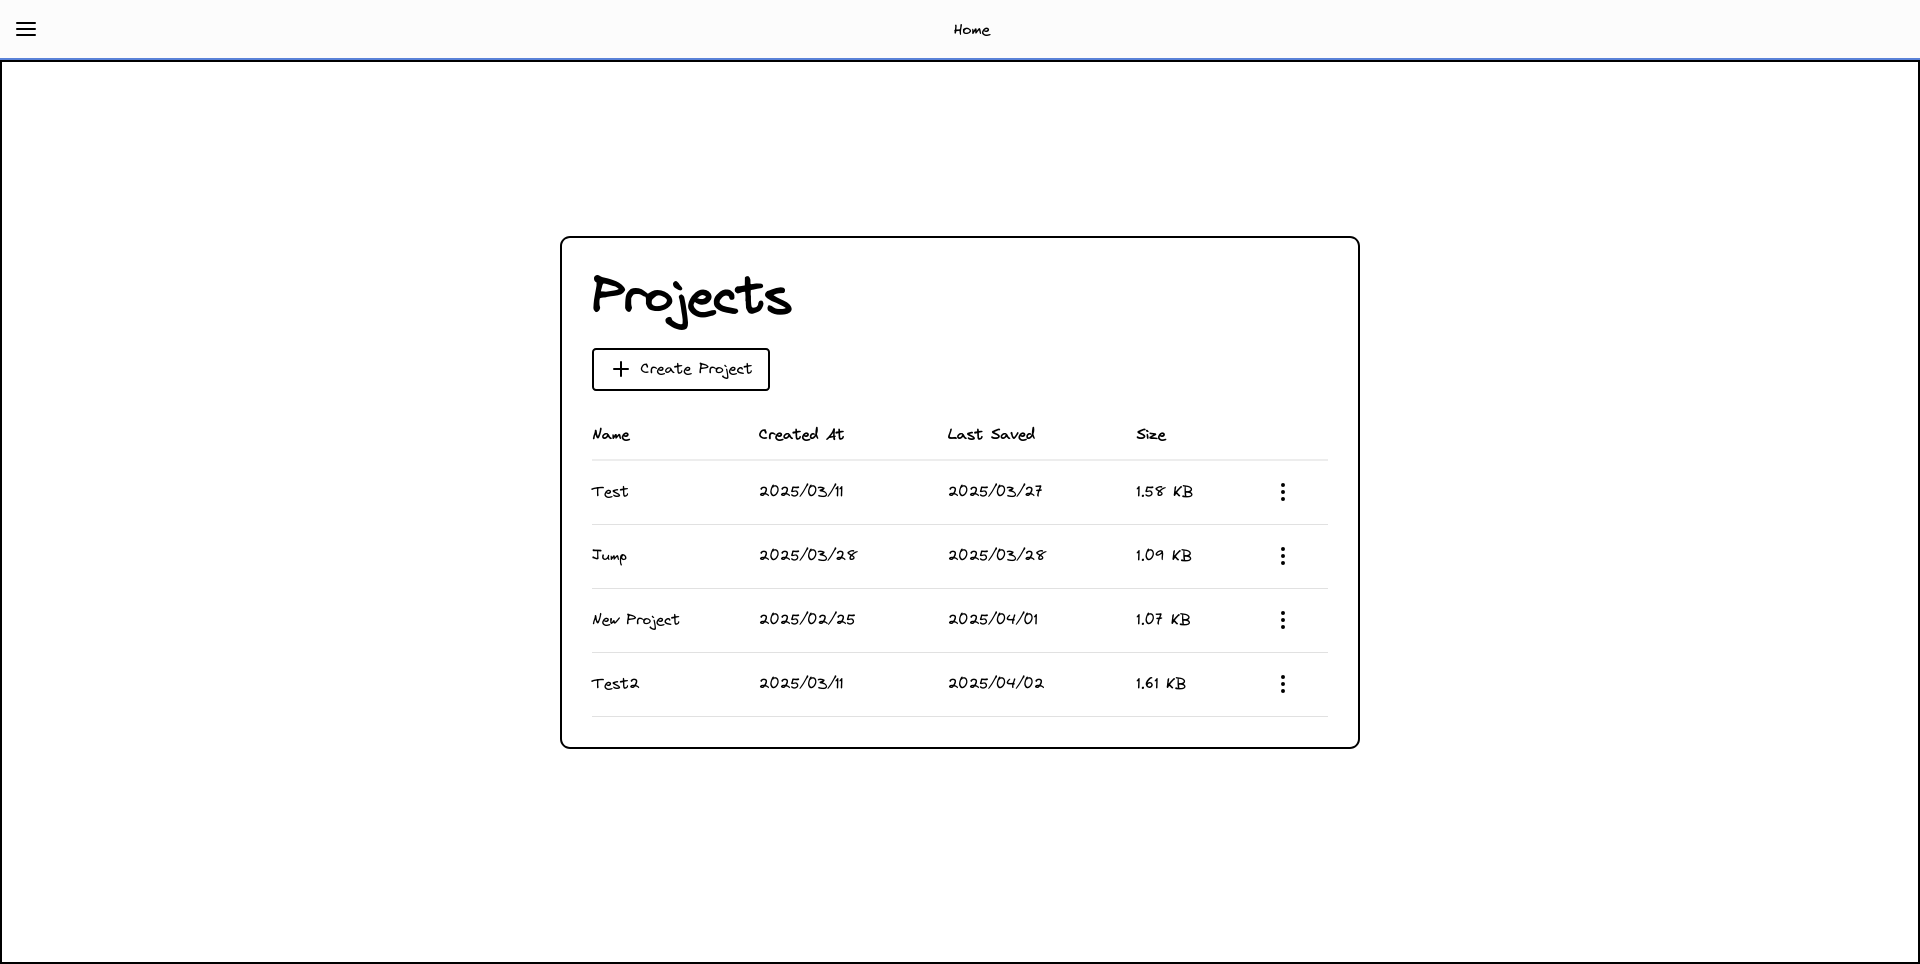
\includegraphics[width=1\textwidth]{assets/images/projects_list_wireframe.png}
    \caption{Wireframe of the Projects List Page}
    \label{fig:projects_list_wireframe}
\end{figure}

\section{Instruction Configuration Page}
The instruction configuration page enables users to define custom instructions for the simulator. Users can add, edit, or delete instructions directly from this page. Since each processor architecture has its own unique instruction set, users must first select the architecture they wish to configure. Once selected, a list of default instructions for the chosen architecture, along with any custom instructions previously defined by the user, will be displayed. Further on that will be a section for editing the selected instruction, which will include all the fields defined in Table \ref{tab:instruction_config}. 



\begin{figure}[H]
    \centering
    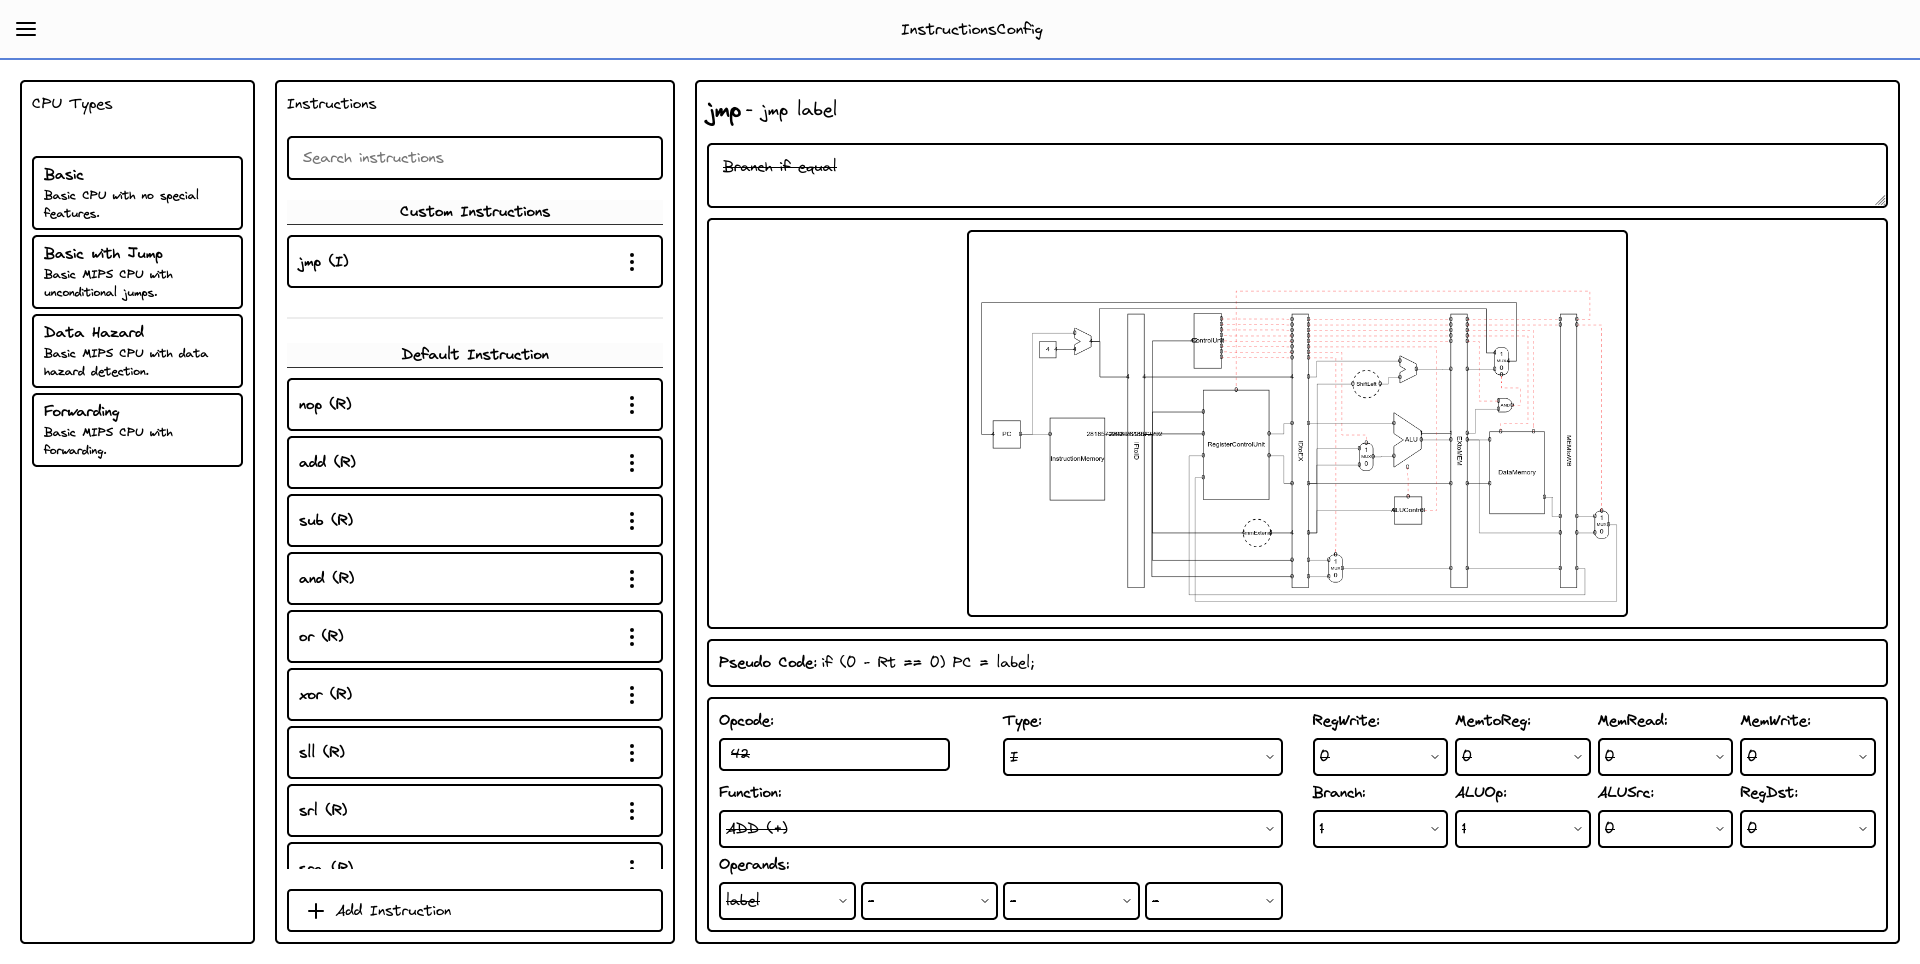
\includegraphics[width=1\textwidth]{assets/images/instruction_config_wireframe.png}
    \caption{Wireframe of the Instruction Configuration Page}
    \label{fig:instruction_config_wireframe}
\end{figure}

\section{Simulator Page}
The simulator page serves as the primary interface of the application, showcasing the pipeline diagram, memory, registers, and controls for managing the simulation (start, pause, step, and reset). Each component, including the pipeline diagram, editor, memory, and registers, will be movable and resizable, allowing users to customize the layout to their preference. The pipeline diagram will take center stage, providing a visual representation of the pipeline's current state and the instructions being executed. Memory and registers will be displayed in a straightforward table format, reflecting their current states. Controls for managing the simulation will be positioned above the editor. The problems tab will display any errors or warnings, and additionally, a searchable instruction list will be available, showing all instructions currently loaded into the simulator.

\begin{figure}[H]
    \centering
    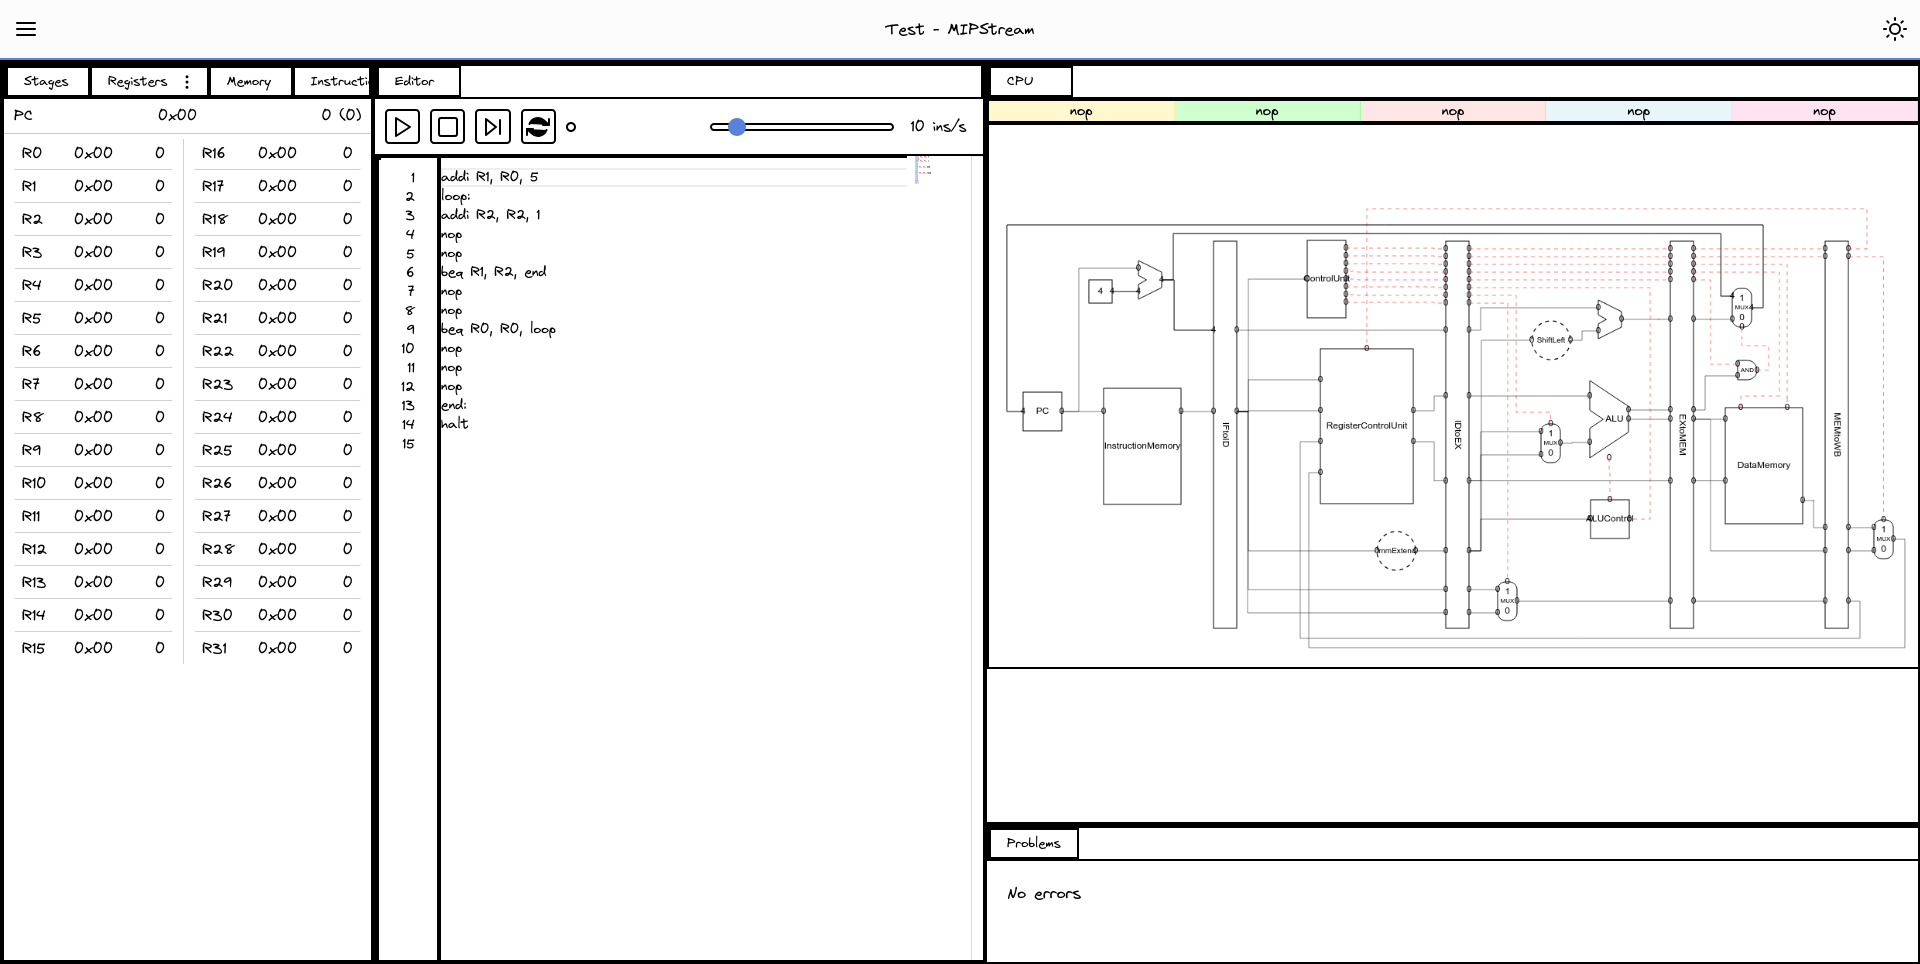
\includegraphics[width=1\textwidth]{assets/images/simulator_wireframe.png}
    \caption{Wireframe of the Simulator Page}
    \label{fig:simulator_wireframe}
\end{figure}


\subsection{Editor}
For a simple and feature-full implementation of an editor for the assembly code, the Monaco Editor will be used. It is a powerful code editor that is based on Visual Studio Code's editor. It supports syntax highlighting, code completion, error checking, and many other features that are essential for a code editor. The Monaco Editor is also highly customizable, allowing for the addition of custom themes, keybindings, and other features. It is also lightweight and fast, making it ideal for a web-based application.

\subsection{Pipeline Diagram}
The pipeline diagram should be implemented using the Canvas API. The Canvas API is a powerful and flexible way to draw graphics on the web. It allows for the creation of complex shapes, animations, and interactions. The Canvas API is also highly performant, making it ideal for a simulation application. The pipeline diagram will be drawn on a canvas element, which will be updated in real-time as the simulation progresses. This will allow for a smooth and responsive user experience. 
As opposed to using SVG, which is a markup language for describing two-dimensional graphics, implementing the diagram with the Canvas API will be more time-consuming and complex in the short term. But when it comes to ease of adding other features and more diagrams for different CPU architectures, the Canvas API will be a much better choice in the long run.

The pipeline diagram will work by receiving a configuration of the components and connections, then drawing them. This makes it easier to edit the diagram as it will have a specially designed logic for this use case. To update its state, it should ideally be tied directly to the cpu's state, so that it can be updated in real-time. This will allow for a smooth and responsive user experience. Hovering over any component or port should trigger an information box popup that will show the current state of the component or port. And the values of each port should be displayed in the diagram, so that the user can see the current state of the pipeline at a glance.

% Figure
\begin{figure}[H]
    \centering
    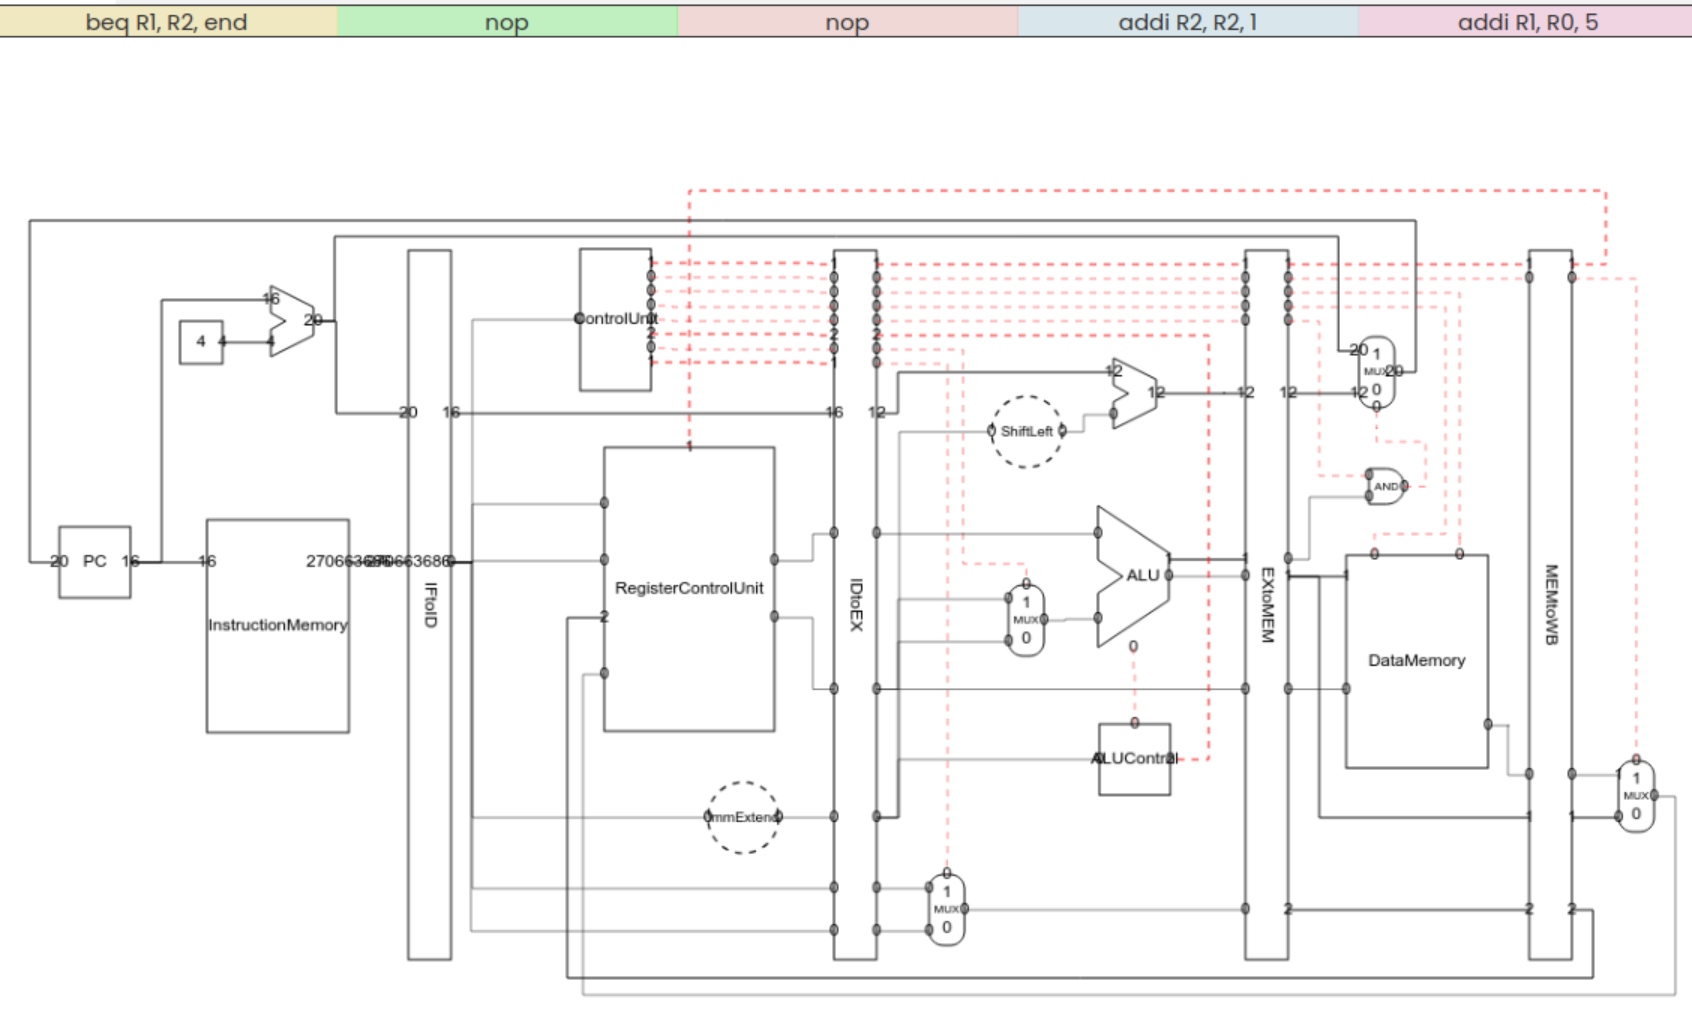
\includegraphics[width=1\textwidth]{assets/images/pipeline_diagram_example.png}
    \caption{Example of a Pipeline Diagram}
    \label{fig:pipeline_diagram_example}
\end{figure}

\subsection{Memory and Register Display}
The memory and register display should both be implemented as a simple table that shows the current state of the memory and registers. The table should be updated in real-time as the simulation progresses, so that the user can see the current state of the memory and registers at a glance. The table should also allow for editing of the values when clicking on them, so that the user can modify the state of the memory and registers during the simulation. This will allow for a more interactive and engaging user experience.

\subsection{Error Handling}
Error handling is an important part of any application, and the simulator is no exception. The simulator should be able to handle errors gracefully and provide feedback to the user in case of errors. This includes syntax errors in the assembly code, invalid instructions, and other errors that may occur during the simulation or assembly. The error handling should be implemented in a way that allows for easy debugging and troubleshooting. The error should be shown both in the editor at the line where the error occurred and in a separate error log that shows all errors.

\subsection{Settings}
The settings will be accessible through the top-left hamburger menu of the application. They should be presented as a straightforward form, enabling users to customize various aspects of the simulator. This includes selecting the default CPU model, adjusting UI themes, and configuring other relevant preferences. The settings will be saved in the browser's local storage, ensuring they persist across sessions and provide a consistent user experience.


